% meta.concepts: particles; 2D equilibrium; force components
% meta.tags: realistic
% acknowledge: Peter Seiler & Luke Melander graciously shared Spring 2019 course material

The figure below shows a hanging robot lamp and a simplified diagram of the hanging robot. The weight of the robot is $W = 4N$. The tension $T$ in each robot arm acts at an angle $\beta = 25^\circ$ from vertical. What is the tension $T$ so that the total vertical force from the two arms balances the downward weight $W$ of the robot?

\begin{figure}[ht!]
  \centering
  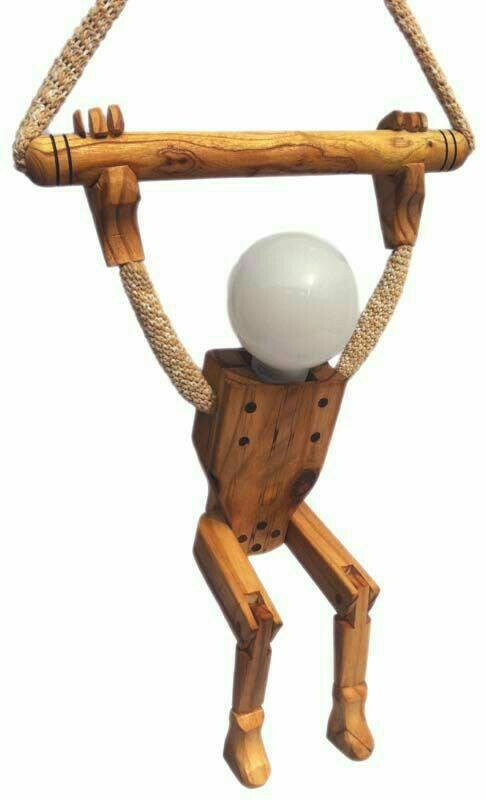
\includegraphics[height=1.8in]{robot-lamp.png}
  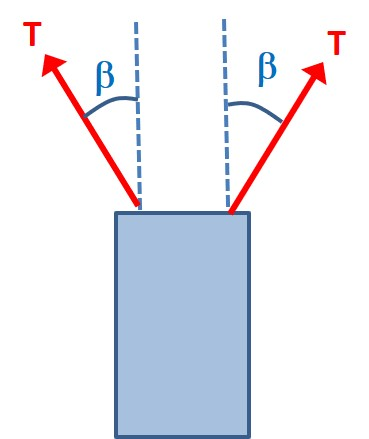
\includegraphics[height=1.8in]{robot-lamp-diagram.png}
\end{figure}

\vspace{.5cm}
\rule{\textwidth}{.4pt}
\vspace{.5cm}
\textbf{Solution:}
\begin{figure}[ht!]
  \centering
  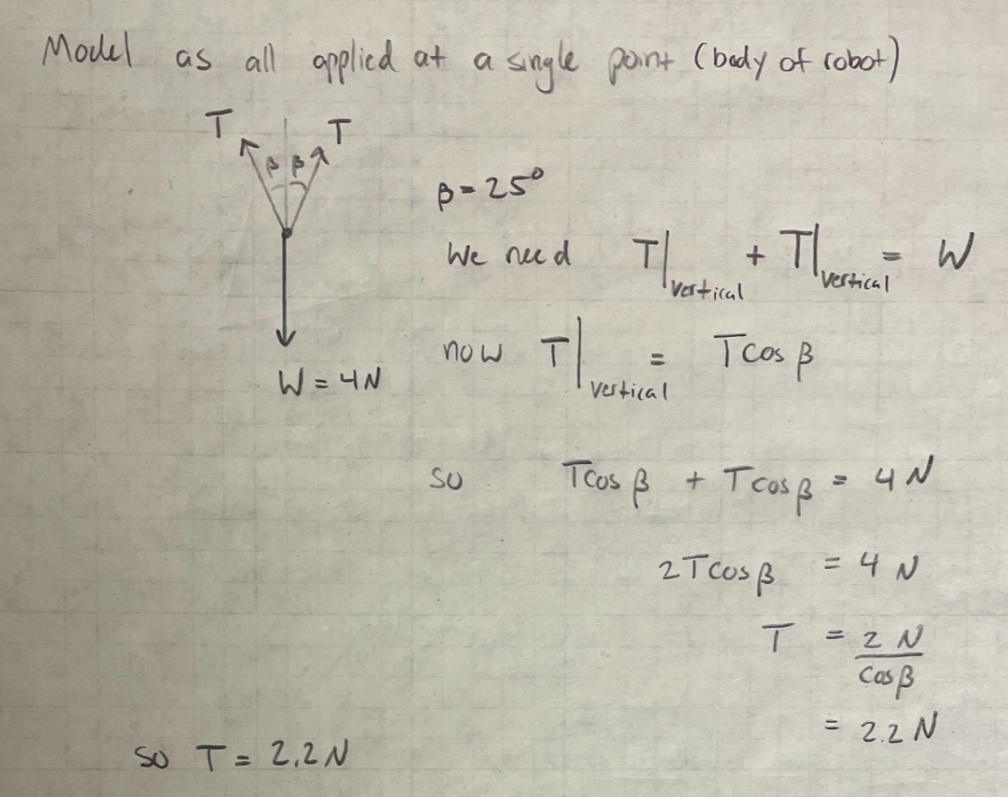
\includegraphics[width=0.9\textwidth]{soln.png}
\end{figure}

